% !TEX root = ../main.tex
\section{Method}
\label{sec:method}
Let $q$ be a problem and $a$ its solution. A frozen teacher supplies contextual token representations for supervised training. We train a conditional flow model over compressed representations of the complete answer, and a token decoder that shares the denoising backbone. Figure~\ref{fig:pipeline} summarizes the stages.

\begin{figure}[t]
\centering
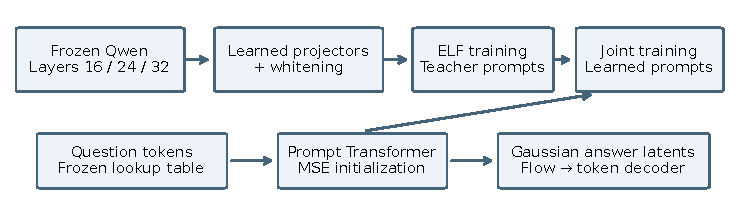
\includegraphics[width=\linewidth]{figures/pipeline.pdf}
\caption{Training and inference. Teacher activations define the latent targets. The prompt Transformer first imitates teacher prompt states, then adapts jointly with a mature ELF model. At inference, only the prompt encoder, denoiser, and terminal token decoder are used; the teacher Transformer is absent.}
\label{fig:pipeline}
\end{figure}

\subsection{Teacher-trained, whitened multilayer representations}
For a token position $j$, write the teacher's post-block activation as $h_j^{(\ell)}\in\R^{2560}$ for $\ell\in\{16,24,32\}$. Each layer is compressed separately:
\begin{equation}
 x_j^{(\ell)}=(h_j^{(\ell)}-\mu_\ell)E_\ell,
 \qquad x_j=[x_j^{(16)},x_j^{(24)},x_j^{(32)}]\in\R^{1024},
 \label{eq:encoding}
\end{equation}
with dimensions $(256,256,512)$. A layer-wise CKA analysis \citep{cka} motivates including layer 16, after which layers 24 and 32 provide regularly spaced deeper representations (Appendix~\ref{app:cka}).

We learn each projector through an independent reconstruction intervention. A trainable decoder maps the compressed state back to the teacher width, $\widehat h_j^{(\ell)}=\mu_\ell+x_j^{(\ell)}D_\ell^\top$. The frozen teacher suffix then produces a next-token distribution $p_{\ell}$, which is trained against the clean teacher distribution $p_{\rm T}$:
\begin{equation}
 \mathcal L_{\rm proj}^{(\ell)}
 =\E_{q,a,j}\left[-\sum_{v\in\mathcal V}p_{\rm T}(v\mid q,a_{\le j})
 \log p_{\ell}(v\mid q,a_{\le j})\right].
 \label{eq:projector}
\end{equation}
Only assistant-content activations are replaced, one layer at a time; the teacher remains frozen. This objective preserves predictive behavior through the remaining teacher layers instead of optimizing reconstruction error alone.

Covariance whitening fixes the scale of the latent coordinates. Let $\widetilde C_\ell$ denote a regularized activation covariance. We use $E_\ell^\top\widetilde C_\ell E_\ell=I$, with a differentiable orthonormal-basis parameterization described in Appendix~\ref{app:projectors}. This prevents the representation from reducing a squared-error objective merely by shrinking its coordinates. Whitening is per layer: it does not assume that different layers are uncorrelated. Once fitted, the representation is fixed during ELF training.

\subsection{Conditional denoising and terminal decoding}
\label{sec:denoising}
We follow the continuous embedding-space formulation of ELF \citep{elf} and flow matching \citep{flowmatching}. For answer latents $x$ and Gaussian noise $\epsilon$, training interpolates
\begin{equation}
 z_t=t x+(1-t)\sigma\epsilon,\quad
 t\sim\LN(-1.5,0.8^2),\quad \epsilon\sim\mathcal N(0,I),\quad \sigma=2.
\end{equation}
The bidirectional Transformer $F_\theta$ predicts the clean endpoint. With prompt condition $c$ and answer self-conditioning $s$, the corresponding velocity is
\begin{equation}
 v_\theta(z_t,t,c,s)=\frac{F_\theta(z_t,t,c,s)-z_t}{\Delta_t},
 \qquad \Delta_t=\max(1-t,0.05).
\end{equation}
The data target uses the same denominator. We inherit ELF's self-conditioning and self-conditioning classifier-free guidance (SCCFG); auxiliary target passes are detached. Prompt positions are restored to the clean condition and excluded from the loss.

A row uses the denoising objective with probability $0.8$ and token-decoder cross-entropy with probability $0.2$. The decoder receives noisy clean latents, uses the same Transformer backbone in decoder mode, and predicts tokens at their own positions. For response mask $M$ and row indicator $b_r\sim\mathrm{Bernoulli}(0.2)$, the local objective is
\begin{equation}
 \mathcal L_{\rm ELF}=
 \frac{\sum_{rj}M_{rj}\left[
 (1-b_r)\|v_{\theta,rj}-\widetilde v^*_{rj}\|_2^2/1024
 +b_r\CE(H_\theta(z^{\rm dec})_{rj},y_{rj})\right]}{\sum_{rj}M_{rj}}.
 \label{eq:elf}
\end{equation}
Here $\widetilde v^*$ is the SCCFG-adjusted target. The mask includes the answer's terminal token and excludes padding. Appendix~\ref{app:objective} gives the decoder corruption and guidance details.

\subsection{Staged prompt conditioning}
\label{sec:prompt}
Original ELF conditions on clean contextual embeddings from a frozen T5 encoder \citep{elf}. FMLM+ instead supplies clean one-hot prompt states to the denoising Transformer, which contextualizes the prompt together with the noisy answer without a separate prompt encoder \citep{posterior}. We retain ELF's contextual conditioning interface, but learn a smaller prompt Transformer to replace the Qwen teacher at inference.

Initially, the denoiser conditions on projected teacher activations of the question alone. A separate six-layer bidirectional prompt Transformer $P_\phi$ maps frozen Qwen token embeddings through a $2560\!\to\!512\!\to\!d_{\rm model}$ frontend and a 1,024-dimensional output. It first imitates the teacher prompt targets using an equally weighted per-question MSE:
\begin{equation}
 \mathcal L_{\rm prompt}=\E_q\left[
 \frac{1}{1024L_q}\sum_{j=1}^{L_q}
 \|P_\phi(q)_j-c_{{\rm T},j}(q)\|_2^2\right].
\end{equation}
After 12 denoiser epochs, we substitute $P_\phi(q)$ for the teacher prompt and continue training both $\theta$ and $\phi$ under Eq.~\eqref{eq:elf}. Answer targets remain fixed; no prompt-imitation term is added during joint training. Gradients through the main conditional forward adapt the prompt representation to the downstream objective.
At inference, $P_\phi(q)$ is computed once and reused throughout denoising. The frozen Qwen token lookup is retained, but none of Qwen's Transformer layers is evaluated.

\subsection{Layer-specific inference clocks}
\label{sec:clocks}
Training uses a shared scalar time. At inference, each latent group has a clock $t_\ell=f_\ell(\tau)=\tau^{\gamma_\ell}$. We use $\bm\gamma=\asyncclock$ in layer order $(16,24,32)$. The scalar time embedder is reused for each group and its embeddings are averaged. Euler integration follows
\begin{equation}
 z^{(\ell)}_{k+1}=z^{(\ell)}_k+
 (\tau_{k+1}-\tau_k) f'_\ell(\tau_k)
 \frac{\widehat x^{(\ell)}_k-z^{(\ell)}_k}{\max(1-f_\ell(\tau_k),0.05)}.
 \label{eq:sampler}
\end{equation}
The grid is formed from logit-normal quantiles, with endpoints zero and one. Recurrent self-conditioning carries the previous clean prediction forward, and prompt states are restored at each step. The final latent state is decoded once to a complete token sequence. All reported generations use SCCFG scale two and greedy terminal decoding. A denoising-step budget counts integration steps; the terminal decoder is an additional backbone call.

\subsection{Reward-based fine-tuning}
\label{sec:nft}
We adapt DiffusionNFT \citep{diffusionnft}, which optimizes a diffusion policy through forward-process training rather than differentiating through generation trajectories. Each prompt group contains 15 old-policy samples and one reference solution. Correct generations receive reward $0.75$, incorrect generations zero, and the reference solution one. We discard groups whose 15 generated answers are all correct, center rewards within each retained group, and normalize using the standard deviation of retained raw rewards.

The resulting coefficients weight positive and negative policy residuals, with an additional penalty toward a fixed reference policy. The prompt encoder and denoising parameters are updated; decoder-only parameters remain frozen. Rollouts use 32 steps with synchronous identity clocks. Our implementation adds the reference-solution anchor, all-correct filtering, token-mask-aware normalization, and a detached SCCFG-compatible velocity construction. Appendix~\ref{app:nft} specifies the exact loss and sampling procedure.
